% !TeX spellcheck = cs_CZ
%{\tikzset{external/prefix={tikz/FYZI/}}
% \tikzset{external/figure name/.add={ch36_}{}}
%---------------------------------------------------------------------------------------------------
% file fey1ch36.tex
%---------------------------------------------------------------------------------------------------
%=========================== Kapitola: Mechanizmus vidění ==========================================
\chapter{Mechanizmus vidění}\label{fyz:IchapXXXVI}
\minitoc
  \section{Barevný vjem}\label{fyz:IchapXXXVIsecI}
  \section{Fyziologie oka}\label{fyz:IchapXXXVIsecII}
  \section{Tyčinky}\label{fyz:IchapXXXVIsecIII}
  \section{Složené oko hmyzu}\label{fyz:IchapXXXVIsecIV}
  \section{Jiné oči}\label{fyz:IchapXXXVIsecV}

  \begin{figure}[ht!] %\ref{fyz:fig489}
    \centering
    
\includegraphics[width=0.6\linewidth]{fyz_fig489.pdf}
    \caption{
             (\cite[s.~697]{Feynman01})}
    \label{fyz:fig489}
  \end{figure}

  \begin{figure}[ht!] %\ref{fyz:fig490}
    \centering
    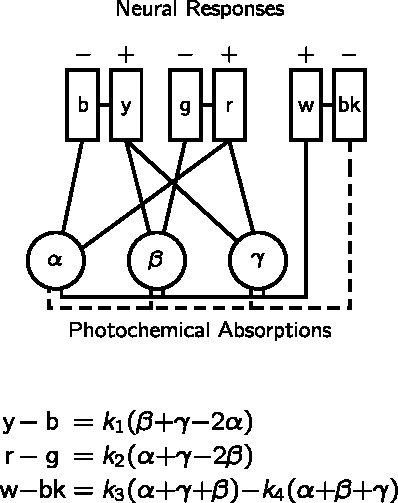
\includegraphics[width=0.6\linewidth]{fyz_fig490.pdf}
    \caption{
             (\cite[s.~697]{Feynman01})}
    \label{fyz:fig490}
  \end{figure}

  \begin{figure}[ht!] %\ref{fyz:fig491}
    \centering
    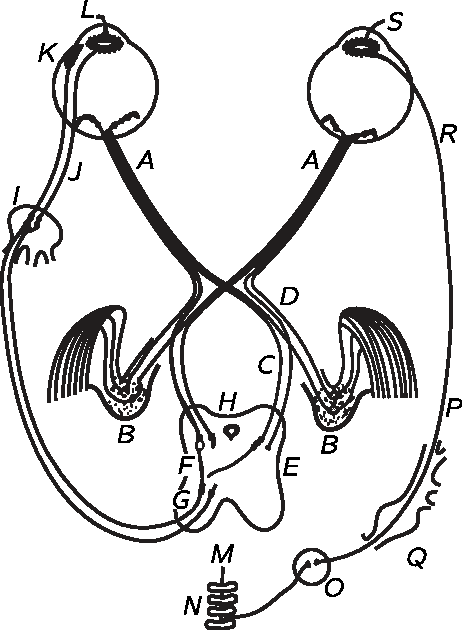
\includegraphics[width=0.6\linewidth]{fyz_fig491.pdf}
    \caption{
             (\cite[s.~697]{Feynman01})}
    \label{fyz:fig491}
  \end{figure}

  \begin{figure}[ht!] %\ref{fyz:fig492}
    \centering
    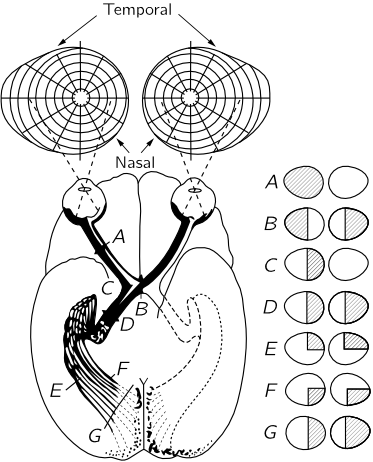
\includegraphics[width=0.8\linewidth]{fyz_fig492.png}
    \caption{
             (\cite[s.~697]{Feynman01})}
    \label{fyz:fig492}
  \end{figure}

  \begin{figure}[ht!] %\ref{fyz:fig493}
    \centering
    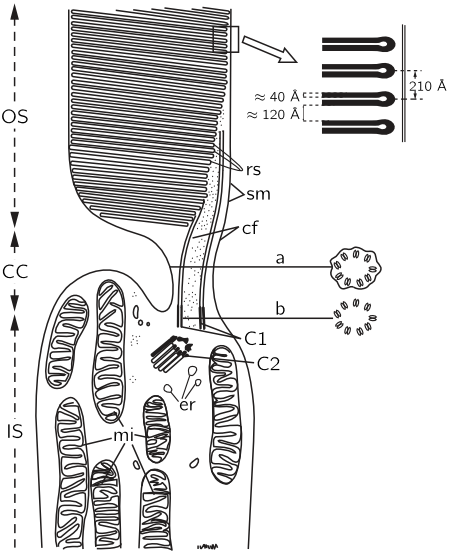
\includegraphics[width=0.8\linewidth]{fyz_fig493.png}
    \caption{
             (\cite[s.~697]{Feynman01})}
    \label{fyz:fig493}
  \end{figure}

  \begin{figure}[ht!] %\ref{fyz:fig494}
    \centering
    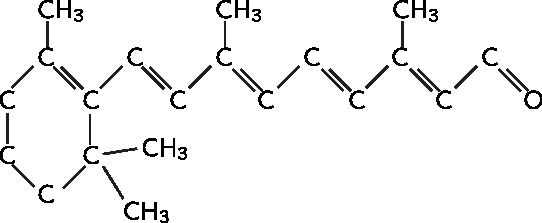
\includegraphics[width=0.6\linewidth]{fyz_fig494.pdf}
    \caption{
             (\cite[s.~697]{Feynman01})}
    \label{fyz:fig494}
  \end{figure}

  \begin{figure}[ht!] %\ref{fyz:fig495}
    \centering
    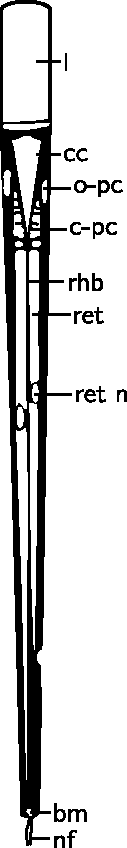
\includegraphics[width=0.2\linewidth]{fyz_fig495.pdf}
    \caption{
             (\cite[s.~697]{Feynman01})}
    \label{fyz:fig495}
  \end{figure}

  \begin{figure}[ht!] %\ref{fyz:fig496}
    \centering
    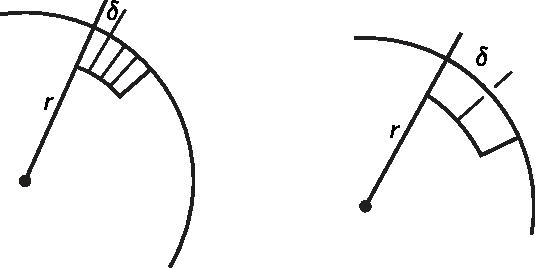
\includegraphics[width=0.6\linewidth]{fyz_fig496.pdf}
    \caption{
             (\cite[s.~697]{Feynman01})}
    \label{fyz:fig496}
  \end{figure}

  \begin{figure}[ht!] %\ref{fyz:fig497}
    \centering
    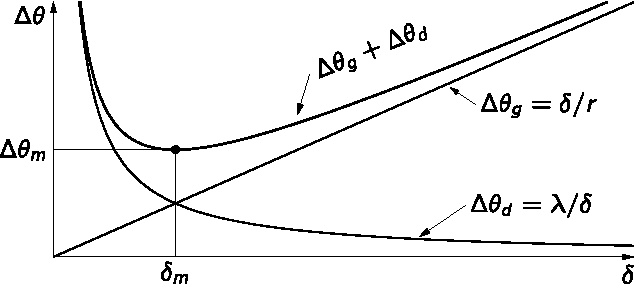
\includegraphics[width=0.6\linewidth]{fyz_fig497.pdf}
    \caption{
             (\cite[s.~697]{Feynman01})}
    \label{fyz:fig497}
  \end{figure}

  \begin{figure}[ht!] %\ref{fyz:fig498}
    \centering
    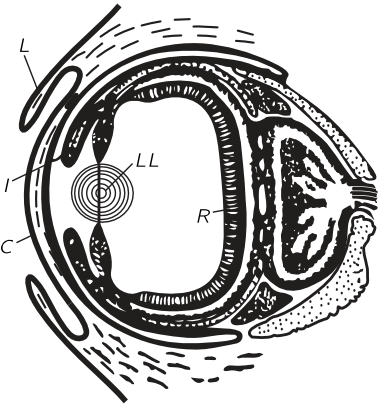
\includegraphics[width=0.6\linewidth]{fyz_fig498.png}
    \caption{
             (\cite[s.~697]{Feynman01})}
    \label{fyz:fig498}
  \end{figure}

  \begin{figure}[hb!] %\ref{fyz:fig499}
    \centering
    \begin{tabular}{c}
     \subfloat[ ]{\label{fyz:fig499a}
       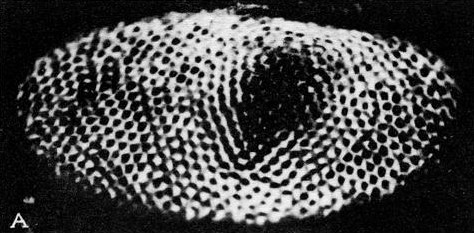
\includegraphics[width=0.6\linewidth]{fyz_fig499a.jpg}} \\
     \subfloat[ ]{\label{fyz:fig499b}
       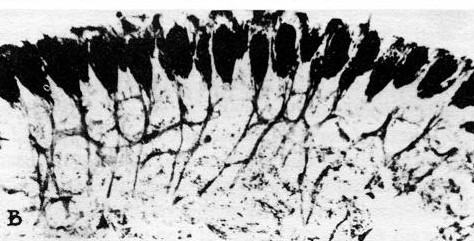
\includegraphics[width=0.6\linewidth]{fyz_fig499b.jpg}}
    \end{tabular}
    \caption{
             (\cite[s.~601]{Feynman01}).}
    \label{fyz:fig499}
  \end{figure}

  \begin{figure}[hb!] %\ref{fyz:fig500}
    \centering
    \begin{tabular}{c}
     \subfloat[ ]{\label{fyz:fig500a}
       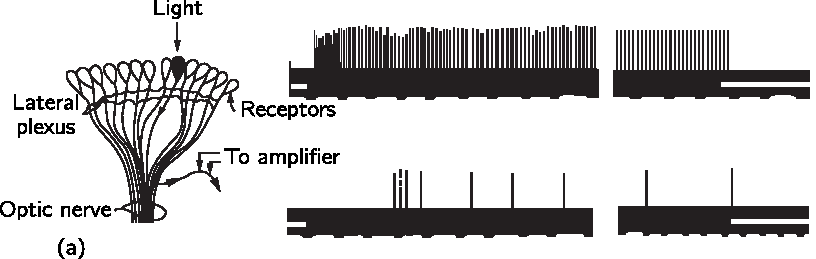
\includegraphics[width=0.9\linewidth]{fyz_fig500a.pdf}}  \\
     \subfloat[ ]{\label{fyz:fig500b}
       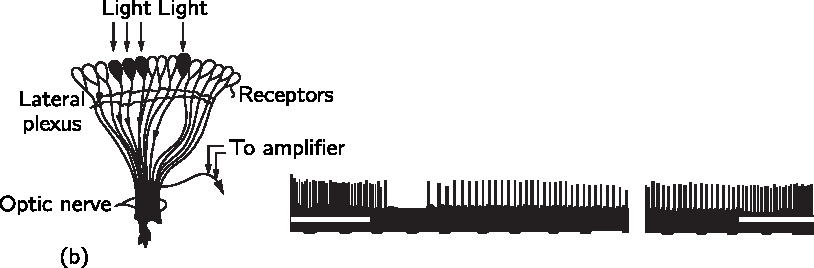
\includegraphics[width=0.9\linewidth]{fyz_fig500b.pdf}}  
    \end{tabular}
    \caption{
             (\cite[s.~601]{Feynman01}).}
    \label{fyz:fig500}
  \end{figure}

  \begin{figure}[ht!] %\ref{fyz:fig501}
    \centering
    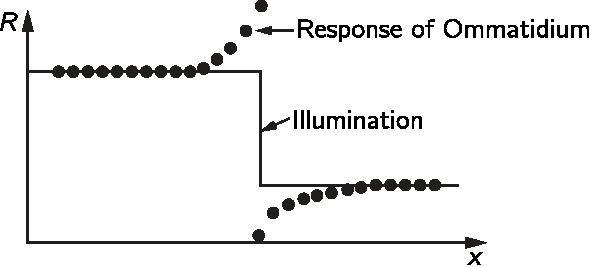
\includegraphics[width=0.6\linewidth]{fyz_fig501.pdf}
    \caption{
             (\cite[s.~697]{Feynman01})}
    \label{fyz:fig501}
  \end{figure}

  \begin{figure}[ht!] %\ref{fyz:fig502}
    \centering
    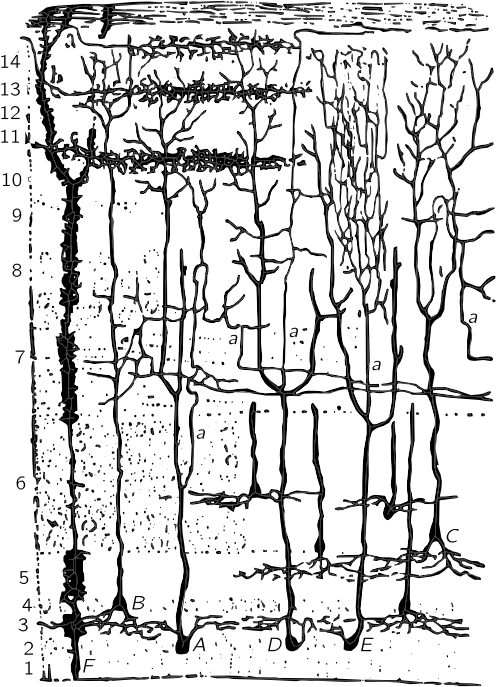
\includegraphics[width=0.8\linewidth]{fyz_fig502.png}
    \caption{
             (\cite[s.~697]{Feynman01})}
    \label{fyz:fig502}
  \end{figure}
  
%} %tikzset
%---------------------------------------------------------------------------------------------------
%\printbibliography[title={Seznam literatury},heading=subbibliography]
\addcontentsline{toc}{section}{Seznam literatury}